
\documentclass[11pt]{article}

% Language setting
\usepackage[turkish]{babel}
\usepackage{pythonhighlight}

\usepackage[a4paper,top=2cm,bottom=2cm,left=2cm,right=2cm,marginparwidth=2cm]{geometry}

% Useful packages
\usepackage{amsmath}
\usepackage{graphicx}
\usepackage[colorlinks=true, allcolors=blue]{hyperref}
\usepackage{verbatim}
\usepackage{fancyhdr} % for header and footer
\usepackage{titlesec}
\usepackage{parskip}

\setlength{\parindent}{0pt}

\titleformat{\subsection}[runin]{\bfseries}{\thesubsection}{1em}{}

\pagestyle{fancy} % activate the custom header/footer

% define the header/footer contents
\lhead{\small{23BLM-4014 Yapay Sinir Ağları Ara Sınav Soru ve Cevap Kağıdı}}
\rhead{\small{Dr. Ulya Bayram}}
\lfoot{}
\rfoot{}

% remove header/footer on first page
\fancypagestyle{firstpage}{
  \lhead{}
  \rhead{}
  \lfoot{}
  \rfoot{\thepage}
}
 

\title{Çanakkale Onsekiz Mart Üniversitesi, Mühendislik Fakültesi, Bilgisayar Mühendisliği Akademik Dönem 2022-2023\\
Ders: BLM-4014 Yapay Sinir Ağları/Bahar Dönemi\\ 
ARA SINAV SORU VE CEVAP KAĞIDI\\
Dersi Veren Öğretim Elemanı: Dr. Öğretim Üyesi Ulya Bayram}
\author{%
\begin{minipage}{\textwidth}
\raggedright
Öğrenci Adı Soyadı: Hilal Solak\\ % Adınızı soyadınızı ve öğrenci numaranızı noktaların yerine yazın
Öğrenci No: 190401020
\end{minipage}%
}

\date{14 Nisan 2023}

\begin{document}
\maketitle

\vspace{-.5in}
\section*{Açıklamalar:}
\begin{itemize}
    \item Vizeyi çözüp, üzerinde aynı sorular, sizin cevaplar ve sonuçlar olan versiyonunu bu formatta PDF olarak, Teams üzerinden açtığım assignment kısmına yüklemeniz gerekiyor. Bu bahsi geçen PDF'i oluşturmak için LaTeX kullandıysanız, tex dosyasının da yer aldığı Github linkini de ödevin en başına (aşağı url olarak) eklerseniz bonus 5 Puan! (Tavsiye: Overleaf)
    \item Çözümlerde ya da çözümlerin kontrolünü yapmada internetten faydalanmak, ChatGPT gibi servisleri kullanmak serbest. Fakat, herkesin çözümü kendi emeğinden oluşmak zorunda. Çözümlerinizi, cevaplarınızı aşağıda belirttiğim tarih ve saate kadar kimseyle paylaşmayınız. 
    \item Kopyayı önlemek için Github repository'lerinizin hiçbirini \textbf{14 Nisan 2023, saat 15:00'a kadar halka açık (public) yapmayınız!} (Assignment son yükleme saati 13:00 ama internet bağlantısı sorunları olabilir diye en fazla ekstra 2 saat daha vaktiniz var. \textbf{Fakat 13:00 - 15:00 arası yüklemelerden -5 puan!}
    \item Ek puan almak için sağlayacağınız tüm Github repository'lerini \textbf{en geç 15 Nisan 2023 15:00'da halka açık (public) yapmış olun linklerden puan alabilmek için!}
    \item \textbf{14 Nisan 2023, saat 15:00'dan sonra gönderilen vizeler değerlendirilmeye alınmayacak, vize notu olarak 0 (sıfır) verilecektir!} Son anda internet bağlantısı gibi sebeplerden sıfır almayı önlemek için assignment kısmından ara ara çözümlerinizi yükleyebilirsiniz yedekleme için. Verilen son tarih/saatte (14 Nisan 2023, saat 15:00) sistemdeki en son yüklü PDF geçerli olacak.
    \item Çözümlerin ve kodların size ait ve özgün olup olmadığını kontrol eden bir algoritma kullanılacaktır. Kopya çektiği belirlenen vizeler otomatikman 0 (sıfır) alacaktır. Bu nedenle çözümlerinizi ve kodlarınızı yukarıda sağladığım gün ve saatlere kadar kimseyle paylaşmayınız.
    \item Bu vizeden alınabilecek en yüksek not 100'dür. Toplam aldığınız puan 100'ü geçerse, aldığınız not 100'e sabitlenecektir.
    \item LaTeX kullanarak PDF oluşturanlar öz geçmişlerine LaTeX bildiklerini de eklemeyi unutmasınlar :)
    \item Bu vizedeki soruların çözümleri ve tex dosyası için istediğiniz kadar sayıda Github repository'si oluşturabilirsiniz. Sadece yukarıda belirttiğim tarihlerde (14 Nisan 2023 saat 15:00 ile 15 Nisan 2023 saat 15:00 arasında) public yapmayı/halka açmayı ve Github profilinizi de öz geçmişinize eklemeyi unutmayın :)
    \item Bilgisayarınıza hiçbir program kurmadan, Overleaf, Google Colab, Kaggle gibi ortamlar üzerinden bu vizeyi tamamlamanız mümkün. İyi çalışmalar!!
\end{itemize}

(Ekstra 5 puan) \url{https://github.com/HilalSolak/Neural_Network_tex}

\newpage
\section{(Toplam 10 Puan) Hopfield Networks:}

\subsection{(2 Puan)} \textbf{ChatGPT’ye size Hopfield Network’ler ile ilgili detaylı bilgi vermesini isteyin. Sorduğunuz soruyu, ChatGPT'nin çıkartığı cevabı aşağı koyun. Bu cevapta anlamadığınız terimleri de ChatGPT’ye sorup, sorduğunuz soruları ve ChatGPT’nin verdiği cevapları da sırayla aşağı koyun.}\\
\textbf{Sorduğum sorular}\\
\textbf{-Hopfield Network’ler ile ilgili detaylı bilgi verir misin?}
 
Hopfield ağları, yapay sinir ağları sınıfına dahil olan ve özellikle asenkronik işleme için kullanılan bir tür geri beslemeli ağdır. Bu ağlar, John Hopfield tarafından 1982 yılında tanıtılmıştır.\\
Hopfield ağları, özellikle bellek işlemlerinde kullanılır. Örneğin, bir Hopfield ağına bir dizi görüntü verilebilir ve ağ, bu görüntüleri hatırlama ve benzer görüntüleri geri çağırma yeteneğine sahip olabilir.\\
Hopfield ağları, birbirleriyle bağlantılı bir dizi nöronu içerir. Bu nöronlar, ikili bir duruma sahiptir: aktif veya pasif. Ağın enerji fonksiyonu, nöronların bağlantılarını ve durumlarını temel alır. Bu fonksiyon, nöronların durumlarını değiştirerek enerji düzeyini azaltmaya çalışır. Bu, ağın belirli bir duruma ulaşması için iteratif bir süreç kullanarak enerji düzeyini minimize etmesi anlamına gelir.\\
Hopfield ağları, hafıza işlevi görebilirler. Örneğin, ağa bir dizi görüntü verildiğinde, ağ, bu görüntüleri belleğinde tutabilir ve benzer görüntüleri hatırlayabilir. Bu, ağın gürültüye dayanıklı olmasını ve kısmi veya hasarlı verileri de hatırlayabilmesini sağlar.\\
Hopfield ağları, özellikle küçük boyutlu veri kümeleri üzerinde iyi sonuçlar verir. Ancak büyük veri kümeleri üzerinde çalışırken performansı düşük olabilir. Bununla birlikte, Hopfield ağları, özellikle bellek işlemleri için kullanılan birçok farklı yapay sinir ağı türü arasında önemli bir yere sahiptir.
Hopfield ağlarının çalışma prensibi, her bir nöronun diğer nöronlarla bağlantılı olduğu ve bu bağlantıların belirli bir ağırlık değeriyle çarpıldığı bir ağın yapısına dayanır. Bu ağırlıklar, bir enerji fonksiyonunu minimize etmek için ayarlanır. Bu enerji fonksiyonu, ağın belirli bir duruma ulaşması için iteratif bir süreç kullanarak enerji düzeyini minimize etmeye çalışır.
Hopfield ağlarının en önemli özelliklerinden biri, herhangi bir girdi verildiğinde ağın bir sonuca ulaşabilmesidir. Yani, ağın bir şekilde "dengelenmesi" ve istenen sonucu bulması sağlanır. Bu özellik, ağın gürültüye dayanıklı olmasını ve kısmi veya hasarlı verileri de de hatırlayabilmesini sağlar.\\
Hopfield ağları, iki farklı modda çalışabilirler: düzenli ve stokastik. Düzenli modda, ağın her zaman aynı sonuçları üretmesi beklenir. Stokastik modda ise, ağın sonuçları rastgele olabilir ve ağın daha esnek olması sağlanır. Stokastik modda, ağın daha yüksek performans göstermesi mümkündür.\\
Hopfield ağları, birçok farklı uygulama alanında kullanılabilir. Örneğin, desen tanıma, veri sıkıştırma ve veri tamamlama gibi alanlarda kullanılabilir. Bunun yanı sıra, Hopfield ağları, enerji hesaplaması, kombinasyon optimizasyonu ve benzeri alanlarda da kullanılabilir.\\
Sonuç olarak, Hopfield ağları, özellikle bellek işlemleri için kullanılan ve hafıza işlevi görebilen bir tür yapay sinir ağıdır.\\
\textbf{-Hopfield ağları neden özellikle küçük boyutlu veri kümeleri üzerinde iyi sonuçlar verir?}\\
Hopfield ağları, özellikle küçük boyutlu veri kümeleri üzerinde iyi sonuçlar verir çünkü bu ağlar, bellek ve hatırlama işlemleri için tasarlanmıştır. Küçük boyutlu veri kümeleri, Hopfield ağlarının depolayabileceği ve hatırlayabileceği nispeten az sayıda öğe içerir.

Hopfield ağları, öğeler arasındaki bağımlılıkları ve benzerlikleri yakalamak için tasarlanmıştır. Küçük boyutlu veri kümeleri, genellikle birbirleriyle bağlantılıdır ve Hopfield ağları bu bağlantıları yakalayabilir. Ayrıca, Hopfield ağları, küçük boyutlu veri kümelerindeki gürültüyü filtreleyebilir ve gürültülü verileri temizleyebilir.

Ancak, büyük veri kümelerinde Hopfield ağlarının performansı düşük olabilir. Büyük veri kümeleri, çok sayıda öğeyi içerir ve Hopfield ağları bu öğeler arasındaki karmaşık bağımlılıkları ve benzerlikleri tespit etmekte zorlanabilir. Ayrıca, büyük veri kümelerindeki gürültü miktarı da artabilir ve Hopfield ağları bu gürültüyü filtrelemekte başarısız olabilir. Bu nedenle, Hopfield ağları büyük veri kümeleri üzerinde çalışırken, özellikle yüksek boyutlu veri kümeleri için daha karmaşık ve özel tekniklerin kullanılması gerekebilir\\

\textbf{-Desen tanıma nedir?}\\
Desen tanıma, bir veri kümesindeki örüntüleri ve yapıları tanımlama ve sınıflandırma işlemidir. Bu işlem, makine öğrenmesi ve yapay zeka teknikleri ile gerçekleştirilir.

Desen tanıma, özellikle görüntü işleme ve işaret işleme gibi alanlarda yaygın olarak kullanılır. Örneğin, bir görüntüdeki nesneleri otomatik olarak tanımlama ve sınıflandırma, tıbbi görüntülerde hastalıkları teşhis etme, el yazısı tanıma, konuşma tanıma, finansal risk yönetimi gibi birçok alanda desen tanıma teknikleri kullanılır.

Desen tanıma, veri kümesindeki özellikleri ve yapıları tanımlayarak, bu özellikleri kullanarak verileri sınıflandırarak ve modeller oluşturarak yapılır. Bu işlem, makine öğrenmesi ve yapay zeka teknikleri ile gerçekleştirilir. Veri kümesindeki özelliklerin ve yapıların doğru bir şekilde tanımlanması, desen tanıma işleminin başarısı için önemlidir.\\
\textbf{Hopfield network ile veri sıkıştırma nasıl yapılır?}\\
Hopfield ağları, veri sıkıştırma için kullanılabilecek bir teknik değildir. Hopfield ağları, bir tür geri beslemeli sinir ağıdır ve özellikle örüntü tanıma ve hatırlama görevleri için kullanılır.

Ancak, Hopfield ağları, özellikle sıkıştırma işleminde kullanılan otomatik kodlayıcılar için bir temel oluşturabilirler. Otomatik kodlayıcılar, veri sıkıştırması için kullanılan derin öğrenme modelleridir. Otomatik kodlayıcılar, öğrenme süreci sırasında, verilerin içindeki önemli özellikleri bulmaya çalışarak, veri boyutunu azaltırlar.

Hopfield ağları, otomatik kodlayıcılar için bir temel oluşturabilir, çünkü bu ağlar, giriş verilerini depolayarak, belirli bir örüntüyü yeniden oluşturmak için kullanılabilirler. Bu özellikleri nedeniyle, Hopfield ağları, sıkıştırma için kullanılacak veri örüntülerini öğrenmek ve daha sonra bu örüntüleri kullanarak sıkıştırılmış verileri yeniden oluşturmak için kullanılabilirler. Ancak, Hopfield ağları, bu amaçla kullanıldığında, sadece küçük boyutlu veri kümeleri için etkili olabilirler.
\textbf{Kullandığım Kaynaklar}

\subsection{(8 Puan)} \textbf{ChatGPT’nin açıklamalarından ne anladığınızı buraya kendi kelimelerinizle özetleyin. Örneğin ``Hopfield Network nedir? Ne işe yarar? Neden bilmemiz gerekir bunu? Gerçek hayatta kullanılıyor mu?'' gibi. Anlamadığınız kısımlar varsa ve ChatGPT’nin açıklamaları yeterli gelmezse internet dahil farklı kaynaklardan araştırıp, bilgilerin doğruluğunu sorgulamakta serbestsiniz. Konuyu doğru anlayıp anlamamanız puana etki edecektir. Kullandığınız kaynakları da belirtin!}

Hopfield ağı, 1980'li yıllarda ilişkisel sinir ağı modelleri üzerine yapılan John Hopfield tarafından tanıtılan spesifik bir tekrarlayan yapay sinir ağıdır. Bu ağlar, birbirleriyle bağlantılı bir dizi nöronu içerir ve ikili bir duruma sahiptir: aktif veya pasif.Ağın enerji fonksiyonu, nöronların bağlantılarına ve durumlarına bağlıdır ve ağın belirli bir duruma gelmesi için enerji seviyesini en aza indirmeye çalışır. Hopfield ağları, hafıza işlevi görebilirler ve özellikle küçük veri kümeleriyle iyi performans gösterir ve depolama işlemleri için kullanılan çeşitli sinir ağları arasında önemli bir yer tutar.\\

Hopfield ağlarının gerçek hayatta kullanımı bulunmaktadır ve yapay sinir ağları arasında bellek işlemleri için kullanılan önemli bir yere sahip teknolojidir. Ayrıca, desen tanıma, veri sıkıştırma, veri tamamlama, enerji hesaplaması, kombinasyon optimizasyonu,şifreleme işlemleri,karakter-desen eşleştirme
,bozuk şekillerin yeniden Oluşturulması,el yazı tanımlama sistemleri gibi birçok uygulama alanında kullanılabilirler.
Bu nedenlerle, Hopfield ağları hakkında bilgi sahibi olmak, yapay zeka ve veri işleme alanlarında çalışanlar için faydalı olabilir.\\

\textbf{Kullandığım Kaynaklar}\\
-\url{https://tr.theastrologypage.com/hopfield-network}\\
-\url{https://medium.com/@batincangurbuz/hopfield-a%C4%9F-modeli-hopfield-network-hn-ccf1548ca432}
\section{(Toplam 10 Puan) Boltzman Machine:}

\subsection{(2 Puan)} \textbf{ChatGPT’ye size Boltzman Machine ilgili detaylı bilgi vermesini isteyin. Sorduğunuz soruyu, ChatGPT'nin çıkartığı cevabı aşağı koyun. Bu cevapta anlamadığınız terimleri de ChatGPT’ye sorup, sorduğunuz soruları ve ChatGPT’nin verdiği cevapları da sırayla aşağı koyun.}\\

\textbf{ Boltzman Machine ilgili detaylı bilgi verir misin?}\\
Boltzmann Machine, yapay sinir ağları alanında bir tür enerji tabanlı olasılık modelidir. Bu model, biyolojik sinir ağlarının çeşitli özelliklerini taklit etmek için tasarlanmıştır. Boltzmann Machine, olasılık teorisi ve istatistiksel mekanik prensiplerini kullanarak, girdileri ve çıktıları arasındaki bağıntıları öğrenmek için kullanılabilir.\\
Boltzmann Machine, bir veya daha fazla gizli katmana sahip, geri beslemeli bir yapay sinir ağıdır. Bu yapay sinir ağı, iki tür nöron içerir: gizli nöronlar ve görünür nöronlar. Gizli nöronlar, girdileri saklayan ve sinir ağındaki örtük kalıpları belirleyen nöronlardır. Görünür nöronlar, ağa girdi olarak sağlanan verileri temsil ederler.\\
Bir Boltzmann Machine, iki aşamalı bir öğrenme sürecine sahiptir. İlk aşama, ağın ağırlıklarının rasgele değerlerle başlatılmasıdır. Daha sonra, ağa bir girdi verilir ve ağ, verileri kullanarak gizli nöronlardaki örtük kalıpları belirlemeye çalışır. Bu aşama, bir "gizli" Boltzmann Machine olarak adlandırılır.\\ 
İkinci aşama, "görünür" Boltzmann Machine olarak adlandırılır ve bu aşamada ağın ağırlıkları, ilk aşamadan gelen öğrenme sonuçlarına dayanarak ayarlanır. Bu aşama, ağın verileri daha iyi öğrenmesine ve daha doğru tahminler yapmasına olanak tanır.\\
Boltzmann Machine, genellikle modelleme, veri analizi ve yapay zeka alanlarında kullanılır. Özellikle, karmaşık problemleri çözmek için kullanılabilir ve derin öğrenme ağlarının temel yapı taşı olarak kabul edilir. Günümüzde, Boltzmann Machine teknolojisi, özellikle doğal dil işleme, nesne tanıma ve yüz tanıma gibi birçok uygulama alanında başarıyla kullanılmaktadır.\\
\textbf{Boltzmann machine olasılık teorisi ve istatistiksel mekanik prensipleri nelerdir?}\\
Boltzmann makinesi, olasılık teorisi ve istatistiksel mekanik prensiplerine dayalı bir modeldir. İlk olarak Ludwig Boltzmann tarafından geliştirilmiştir.

Olasılık teorisi, rastgele olayların matematiksel modellerini ve bunların olasılıklarını inceleyen bir matematik dalıdır. İstatistiksel mekanik ise, maddenin makroskopik özelliklerini atomik ve moleküler düzeydeki davranışlardan türetmek için istatistiksel yöntemleri kullanır.

Boltzmann makinesi, birbirleriyle etkileşim halinde olan bir dizi gizli ve gözlemlenebilir değişken arasındaki ilişkiyi modellemek için kullanılır. Bu değişkenlerin her biri, belirli bir durumu temsil eder. Boltzmann makinesi, bu değişkenlerin olasılık dağılımlarını kullanarak, belirli bir durumun olasılığını tahmin etmek için kullanılır.

Bir Boltzmann makinesi, genellikle enerji fonksiyonu adı verilen bir fonksiyon kullanarak, durumların bir enerji düzeyi ataması yapar. Bu enerji düzeyleri, makine tarafından üretilen olasılık dağılımını belirleyen Boltzmann dağılımı ile ilişkilidir. Boltzmann makinesi, verilen bir veri kümesine göre öğrenir ve modelini iyileştirmek için öğrenme algoritmaları kullanır.

Sonuç olarak, Boltzmann makinesi, olasılık teorisi ve istatistiksel mekanik prensiplerine dayalı bir modeldir ve birbirleriyle etkileşim halinde olan değişkenlerin olasılık dağılımlarını kullanarak, belirli bir durumun olasılığını tahmin etmek için kullanılır.\\
\textbf{Gizli boltzmann machine nedir?}\\
Gizli Boltzmann Makinesi (GBM), makine öğrenmesinde yaygın olarak kullanılan bir yapay sinir ağı türüdür. Temel olarak, GBM, veri setlerindeki özellikleri ve aralarındaki ilişkileri modellemek için kullanılır.

GBM, gözlemlenen verilerin bir alt kümesini gizli (latent) değişkenlerle eşleştirerek çalışır. Bu gizli değişkenler, veriler arasındaki karmaşık ilişkileri temsil ederler ve veri setindeki yapıyı ortaya çıkarmaya yardımcı olurlar. GBM, bu gizli değişkenleri ve gözlemlenen verileri bir enerji fonksiyonu aracılığıyla modeller.

GBM, iki katmandan oluşur: gizli bir katman ve bir görünür (visible) katman. Gizli katman, modelin içindeki gizli değişkenleri temsil ederken, görünür katman, verilerin doğrudan gözlemlendiği katmandır. Bu katmanlar arasındaki bağlantılar, birbirleriyle bağlantılı olan bir dizi ağırlık matrisi ile tanımlanır.

GBM, özellikle boyut azaltma, veri sıkıştırma ve özellik öğrenme gibi uygulamalarda kullanılır. Örneğin, bir GBM, görüntü verilerindeki özellikleri öğrenerek görüntüleri daha az boyutlu bir uzayda temsil edebilir ve bu da veri sıkıştırma uygulamalarında faydalıdır.
\subsection{(8 Puan)} \textbf{ChatGPT’nin açıklamalarından ne anladığınızı buraya kendi kelimelerinizle özetleyin. Örneğin ``Boltzman Machine nedir? Ne işe yarar? Neden bilmemiz gerekir bunu? Gerçek hayatta kullanılıyor mu?'' gibi. Anlamadığınız kısımlar varsa ve ChatGPT’nin açıklamaları yeterli gelmezse internet dahil farklı kaynaklardan araştırıp, bilgilerin doğruluğunu sorgulamakta serbestsiniz. Konuyu doğru anlayıp anlamamanız puana etki edecektir. Kullandığınız kaynakları da belirtin!}\\
Bir Boltzmann makinesi, düğümlerin bazı önyargılarla ikili kararlar aldığı bir tekrarlayan sinir ağı türüdür. Boltzmann makineleri, derin inanç ağları gibi daha karmaşık sistemler yapmak için birbirine bağlanabilir.
Boltzmann makinesi aynı zamanda gizli birimleri olan stokastik bir Hopfield ağı olarak da bilinir.
 Bu ağ, çıktılarına etki eden gizli bir katmanı olan bir tür yapay sinir ağıdır. Bu gizli katman sayesinde, Boltzmann Machine, verilen bir girdiyi yorumlayabilir ve olası sonuçları tahmin edebilir.\\

Boltzmann Machine, unsupervised learning (gözetimsiz öğrenme) adı verilen bir öğrenme türü kullanır. Bu, eğitim verileri için herhangi bir etiketleme veya kategorizasyon gerektirmez. Bu öğrenme türü, birçok gerçek hayat senaryosunda kullanışlıdır, özellikle de büyük miktarda veri olduğunda.\\

Boltzmann Machine'in kullanım alanları arasında özellikle sınıflandırma, veri sıkıştırma, örüntü tanıma, keşif ve tahminleme yer alır. Gerçek hayatta, Boltzmann Machine, finansal piyasa tahmini, ürün önerileri, tıbbi teşhisler, ses ve görüntü tanıma gibi birçok alanda kullanılmaktadır.\\

Boltzmann Machine hakkında bilgi sahibi olmanın önemi, yapay zeka, derin öğrenme ve veri madenciliği gibi alanlarda çalışanlar için oldukça yüksektir. Bu alanlarda çalışanlar, Boltzmann Machine'in çalışma prensiplerini anlayarak, veri analizi ve tahmini yürütmek için kullanabilecekleri güçlü bir araç elde ederler.\\
\textbf{Kullandığım Kaynaklar}\\
-\url{https://tr.theastrologypage.com/boltzmann-machine}\\
-\url{https://medium.com/@batincangurbuz/boltzman-makinesi-boltzmann-machines-bm-ve-k%C4%B1s%C4%B1tlanm%C4%B1%C5%9F-boltzmann-makineleri-restricted-boltzmann-6f2e0f839b05}

\section{(Toplam 10 Puan) Markov Assumption ve Markov Chain:}

\subsection{(2 Puan)} \textbf{ChatGPT’ye size Markov assumption ve Markov Chain ilgili detaylı bilgi vermesini isteyin. Sorduğunuz soruyu, ChatGPT'nin çıkartığı cevabı aşağı koyun. Bu cevapta anlamadığınız terimleri de ChatGPT’ye sorup, sorduğunuz soruları ve ChatGPT’nin verdiği cevapları da sırayla aşağı koyun.}\\
\textbf{Markov assumption ve Markov Chain ilgili detaylı bilgi verir misin?}\\
Markov assumption, bir sistemin gelecekteki durumunun, sadece o anki durumuna bağlı olduğunu varsayar. Yani, herhangi bir önceki durum, sadece mevcut durumun belirleyicisi olan bir sonraki duruma geçişi etkilemez. Bu varsayım, birçok uygulama için geçerlidir ve Markov Chain olarak adlandırılan bir modelleme yönteminin temelini oluşturur.

Markov Chain, bir dizi rastgele olayın dizisini modeller. Bu olaylar, her biri belirli bir durumu temsil eden, bir dizi bağlantılı durumdan oluşur. Her bir durum, bir sistemdeki bir değişkenin belirli bir değerini temsil eder. Örneğin, bir finansal piyasanın durumu, bir meteorolojik olayın hava durumu veya bir dildeki bir kelimenin kullanımı olabilir.

Markov Chain'in matematiksel tanımı, her bir durumun olasılık dağılımını tanımlayan bir vektörle ve durumlar arasındaki geçişlerin olasılıklarını tanımlayan bir geçiş matrisiyle yapılır. Bu geçiş matrisi, her bir durumun, diğer durumlara geçme olasılıklarını tanımlar. Örneğin, bir finansal piyasada, bir durumdan diğerine geçme olasılığı, bir hisse senedinin fiyatının artması veya azalması gibi faktörlere bağlı olabilir.

Markov Chain, birbirleriyle bağlantılı durumların bir dizi oluşturduğu bir grafik olarak düşünülebilir. Bu grafikte, her durum bir düğüm ve her geçiş bir kenarla temsil edilir. Markov Chain'in bu grafiksel temsili, belirli bir durumda nelerin mümkün olduğunu ve ne tür geçişlerin mümkün olduğunu gösterir.

Markov Chain, birçok alanda kullanılır. Finansal piyasaların hareketlerinin modellenmesi, meteorolojik olayların tahmini, dil modellemesi, veri sıkıştırma, arama motoru algoritmaları ve çeşitli mühendislik uygulamaları gibi alanlarda Markov Chain sıklıkla kullanılmaktadır. Markov Chain ayrıca, Monte Carlo Simülasyonları ve Bayes Teoremi gibi diğer istatistiksel yöntemlerin temelini de oluşturur.\\
\textbf{Markov chain grafik nasıl oluşturuluyor?}\\
Markov Chain, birbirleriyle bağlantılı durumların bir dizi oluşturduğu bir grafik olarak düşünülebilir. Bu grafik, her bir durumun bir düğüm ve her geçişin bir kenarla temsil edildiği bir yönlü grafiktir. Grafik oluşturmak için, öncelikle sistemdeki farklı durumlar ve bu durumlar arasındaki geçişler belirlenir. Daha sonra, her bir durum bir düğüm olarak temsil edilir ve her geçiş bir kenarla gösterilir. Geçişlerin olasılıkları, kenarlara eklenen ağırlıklar veya etiketler ile gösterilir. Son olarak, oluşturulan grafik, sistemdeki farklı durumlar ve durumlar arasındaki geçişler hakkında bilgi sağlar.\\
\textbf{Markov assumption nasıl ölçülür?}\\
Markov varsayımı, bir sürecin gelecekteki durumunun, yalnızca mevcut duruma bağlı olduğunu varsayar ve geçmiş durumlardan bağımsız olduğunu kabul eder. Bu varsayım, birçok doğal süreç için geçerlidir ve özellikle zaman serileri analizinde yaygın olarak kullanılır.

Markov varsayımının ölçülmesi, bir sürecin ne kadar zamandır geçerli olduğunu belirlemek için kullanılan bir dizi yöntem vardır. Bu yöntemler, sürecin özellikleri ve uygunluğu açısından farklılık gösterir. En yaygın yöntemler arasında, verilen bir sürecin Markov olup olmadığını belirlemek için gözlemlenebilir verilerin kullanıldığı istatistiksel testler yer alır.

Markov varsayımı, sürecin gelecekteki durumunu yalnızca mevcut duruma bağlı olduğu için, verilerde belirli bir desen veya bağımlılık olup olmadığını belirlemek için kullanılan özel teknikler kullanılarak ölçülebilir. Bu teknikler arasında özyinelemeli analiz ve çapraz geçerlilik yer alır. Bu teknikler, verilerdeki bağımlılık düzeylerini ve süreçlerin Markov olup olmadığını belirlemeye yardımcı olabilir.
\subsection{(8 Puan)} \textbf{ChatGPT’nin açıklamalarından ne anladığınızı buraya kendi kelimelerinizle özetleyin. Örneğin ``Markov assumption ve Markov Chain nedir? Ne işe yarar? Neden bilmemiz gerekir bunu? Gerçek hayatta kullanılıyor mu?'' gibi. Anlamadığınız kısımlar varsa ve ChatGPT’nin açıklamaları yeterli gelmezse internet dahil farklı kaynaklardan araştırıp, bilgilerin doğruluğunu sorgulamakta serbestsiniz. Konuyu doğru anlayıp anlamamanız puana etki edecektir. Kullandığınız kaynakları da belirtin!}

Markov assumption (Markov varsayımı), gelecekteki bir olayın yalnızca şu anda bulunulan durumla ilgili olduğunu ve geçmiş durumların önemsiz olduğunu varsayar. Bu varsayımın bir sonucu olarak, Markov Chain (Markov zinciri) olarak adlandırılan bir model ortaya çıkar. Markov Chain, bir sistemin belirli bir zamandaki durumunu tanımlayan bir dizi durum ve bu durumlar arasındaki geçiş olasılıklarını içeren bir matematiksel modeldir.\\
Markov Chain, bir sistemin gelecekteki durumunun sadece o anki durumuna bağlı olduğunu varsayar ve bir dizi rastgele olayın dizisini modeller. Bu olaylar, her biri belirli bir durumu temsil eden bir dizi bağlantılı durumdan oluşur. Matematiksel olarak, her bir durumun olasılık dağılımını tanımlayan bir vektörle ve durumlar arasındaki geçişlerin olasılıklarını tanımlayan bir geçiş matrisiyle yapılır. Markov Chain, birbirleriyle bağlantılı durumların bir dizi oluşturduğu bir grafik olarak düşünülebilir. \\
Markov Chain, birçok alanda kullanılır ve diğer istatistiksel yöntemlerin temelini de oluşturur.Monte Carlo Simülasyonları ve Bayes Teoremi gibi diğer istatistiksel yöntemlerin temelini oluşturur.\\
\textbf{Kullandığım Kaynaklar}\\
- \url{https://en.wikipedia.org/wiki/Markov_chain#:~:text=A%20Markov%20chain%20or%20Markov,the%20state%20of%20affairs%20now.%22}\\
-\url{https://medium.com/@batincangurbuz/markov-zinciri-markov-chain-mc-33cd8a61f6fa}

\section{(Toplam 20 Puan) Feed Forward:}
 
\begin{itemize}
    \item Forward propagation için, input olarak şu X matrisini verin (tensöre çevirmeyi unutmayın):\\
    $X = \begin{bmatrix}
        1 & 2 & 3\\
        4 & 5 & 6
        \end{bmatrix}$
    Satırlar veriler (sample'lar), kolonlar öznitelikler (feature'lar).
    \item Bir adet hidden layer olsun ve içinde tanh aktivasyon fonksiyonu olsun
    \item Hidden layer'da 50 nöron olsun
    \item Bir adet output layer olsun, tek nöronu olsun ve içinde sigmoid aktivasyon fonksiyonu olsun
\end{itemize}

Tanh fonksiyonu:\\
$f(x) = \frac{exp(x) - exp(-x)}{exp(x) + exp(-x)}$
\vspace{.2in}

Sigmoid fonksiyonu:\\
$f(x) = \frac{1}{1 + exp(-x)}$

\vspace{.2in}
 \textbf{Pytorch kütüphanesi ile, ama kütüphanenin hazır aktivasyon fonksiyonlarını kullanmadan, formülünü verdiğim iki aktivasyon fonksiyonunun kodunu ikinci haftada yaptığımız gibi kendiniz yazarak bu yapay sinir ağını oluşturun ve aşağıdaki üç soruya cevap verin.}
 
\subsection{(10 Puan)} \textbf{Yukarıdaki yapay sinir ağını çalıştırmadan önce pytorch için Seed değerini 1 olarak set edin, kodu aşağıdaki kod bloğuna ve altına da sonucu yapıştırın:}

% Latex'de kod koyabilirsiniz python formatında. Aşağıdaki örnekleri silip içine kendi kodunuzu koyun
\begin{python}
import torch

# seed=1 set ediyorum
torch.manual_seed(1)

#Giris tensorunu tanimliyoruz
X = torch.tensor([[1, 2, 3], [4, 5, 6]], dtype=torch.float)

#Yapay sinir agi mimarisini tanimla
class Net(torch.nn.Module):
    def __init__(self):
        super(Net, self).__init__()
        self.hidden = torch.nn.Linear(3, 50)
        self.output = torch.nn.Linear(50, 1)
        
    def tanh(self, x):
        return (torch.exp(x) - torch.exp(-x)) / (torch.exp(x) + torch.exp(-x))
    
    def sigmoid(self, x):
        return 1 / (1 + torch.exp(-x))
        
    def forward(self, x):
        x = self.hidden(x)
        x = self.tanh(x)
        x = self.output(x)
        x = self.sigmoid(x)
        return x

# Yapay sinir agi modelini baslat  
net = Net()

#Yapay sinir agi mimarisini ekrana yazdır
print(net)
#forward propagation gerceklestir.
output = net(X)
# ciktiyi yazdir
print(output)
\end{python}

Net(\\
  (hidden): Linear(in_features=3, out_features=50, bias=True)\\
  (output): Linear(in_features=50, out_features=1, bias=True)
)\\
tensor([[0.4892],
                [0.5566]], grad_fn=<MulBackward0>)

\subsection{(5 Puan)} \textbf{Yukarıdaki yapay sinir ağını çalıştırmadan önce Seed değerini öğrenci numaranız olarak değiştirip, kodu aşağıdaki kod bloğuna ve altına da sonucu yapıştırın:}

\begin{python}
import torch

torch.manual_seed(190401020)#okul numaram

#Giris tensorunu tanimliyoruz
X = torch.tensor([[1, 2, 3], [4, 5, 6]], dtype=torch.float)

#Yapay sinir agi mimarisini tanimla
class Net(torch.nn.Module):
    def __init__(self):
        super(Net, self).__init__()
        self.hidden = torch.nn.Linear(3, 50)
        self.output = torch.nn.Linear(50, 1)
        
    def tanh(self, x):
        return (torch.exp(x) - torch.exp(-x)) / (torch.exp(x) + torch.exp(-x))
    
    def sigmoid(self, x):
        return 1 / (1 + torch.exp(-x))
        
    def forward(self, x):
        x = self.hidden(x)
        x = self.tanh(x)
        x = self.output(x)
        x = self.sigmoid(x)
        return x

# Yapay sinir agi modelini baslat  
net = Net()

#Yapay sinir agi mimarisini ekrana yazdır
print(net)
#forward propagation gerceklestir.
output = net(X)
# ciktiyi yazdir
print(output)
\end{python}

Net(\\
  (hidden): Linear(in_features=3, out_features=50, bias=True)\\
  (output): Linear(in_features=50, out_features=1, bias=True)
)    \\
tensor([[0.5255],
        [0.5461]], grad_fn=<MulBackward0>)

\subsection{(5 Puan)} \textbf{Kodlarınızın ve sonuçlarınızın olduğu jupyter notebook'un Github repository'sindeki linkini aşağıdaki url kısmının içine yapıştırın. İlk sayfada belirttiğim gün ve saate kadar halka açık (public) olmasın:}\\
% size ait Github olmak zorunda, bu vize için ayrı bir github repository'si açıp notebook'u onun içine koyun. Kendine ait olmayıp da arkadaşının notebook'unun linkini paylaşanlar 0 alacak.
4.1 ve 4.2 sorularını bulundurduğum github linki aşağıdadır.\\
\url{https://github.com/HilalSolak/AI_Neural_Networks_Feed-Forward/blob/main/AnswersofQuestions_4.1%26%264.2.ipynb}

\section{(Toplam 40 Puan) Multilayer Perceptron (MLP):} 
\textbf{Bu bölümdeki sorularda benim vize ile beraber paylaştığım Prensesi İyileştir (Cure The Princess) Veri Seti parçaları kullanılacak. Hikaye şöyle (soruyu çözmek için hikaye kısmını okumak zorunda değilsiniz):} 

``Bir zamanlar, çok uzaklarda bir ülkede, ağır bir hastalığa yakalanmış bir prenses yaşarmış. Ülkenin kralı ve kraliçesi onu iyileştirmek için ellerinden gelen her şeyi yapmışlar, ancak denedikleri hiçbir çare işe yaramamış.

Yerel bir grup köylü, herhangi bir hastalığı iyileştirmek için gücü olduğu söylenen bir dizi sihirli malzemeden bahsederek kral ve kraliçeye yaklaşmış. Ancak, köylüler kral ile kraliçeyi, bu malzemelerin etkilerinin patlayıcı olabileceği ve son zamanlarda yaşanan kuraklıklar nedeniyle bu malzemelerden sadece birkaçının herhangi bir zamanda bulunabileceği konusunda uyarmışlar. Ayrıca, sadece deneyimli bir simyacı bu özelliklere sahip patlayıcı ve az bulunan malzemelerin belirli bir kombinasyonunun prensesi iyileştireceğini belirleyebilecekmiş.

Kral ve kraliçe kızlarını kurtarmak için umutsuzlar, bu yüzden ülkedeki en iyi simyacıyı bulmak için yola çıkmışlar. Dağları tepeleri aşmışlar ve nihayet "Yapay Sinir Ağları Uzmanı" olarak bilinen yeni bir sihirli sanatın ustası olarak ün yapmış bir simyacı bulmuşlar.

Simyacı önce köylülerin iddialarını ve her bir malzemenin alınan miktarlarını, ayrıca iyileşmeye yol açıp açmadığını incelemiş. Simyacı biliyormuş ki bu prensesi iyileştirmek için tek bir şansı varmış ve bunu doğru yapmak zorundaymış. (Original source: \url{https://www.kaggle.com/datasets/unmoved/cure-the-princess})

(Buradan itibaren ChatGPT ve Dr. Ulya Bayram'a ait hikayenin devamı)

Simyacı, büyülü bileşenlerin farklı kombinasyonlarını analiz etmek ve denemek için günler harcamış. Sonunda birkaç denemenin ardından prensesi iyileştirecek çeşitli karışım kombinasyonları bulmuş ve bunları bir veri setinde toplamış. Daha sonra bu veri setini eğitim, validasyon ve test setleri olarak üç parçaya ayırmış ve bunun üzerinde bir yapay sinir ağı eğiterek kendi yöntemi ile prensesi iyileştirme ihtimalini hesaplamış ve ikna olunca kral ve kraliçeye haber vermiş. Heyecanlı ve umutlu olan kral ve kraliçe, simyacının prensese hazırladığı ilacı vermesine izin vermiş ve ilaç işe yaramış ve prenses hastalığından kurtulmuş.

Kral ve kraliçe, kızlarının hayatını kurtardığı için simyacıya krallıkta kalması ve çalışmalarına devam etmesi için büyük bir araştırma bütçesi ve çok sayıda GPU'su olan bir server vermiş. İyileşen prenses de kendisini iyileştiren yöntemleri öğrenmeye merak salıp, krallıktaki üniversitenin bilgisayar mühendisliği bölümüne girmiş ve mezun olur olmaz da simyacının yanında, onun araştırma grubunda çalışmaya başlamış. Uzun yıllar birlikte krallıktaki insanlara, hayvanlara ve doğaya faydalı olacak yazılımlar geliştirmişler, ve simyacı emekli olduğunda prenses hem araştırma grubunun hem de krallığın lideri olarak hayatına devam etmiş.

Prenses, kendisini iyileştiren veri setini de, gelecekte onların izinden gidecek bilgisayar mühendisi prensler ve prensesler başkalarına faydalı olabilecek yapay sinir ağları oluşturmayı öğrensinler diye halka açmış ve sınavlarda kullanılmasını salık vermiş.''

\textbf{İki hidden layer'lı bir Multilayer Perceptron (MLP) oluşturun beşinci ve altıncı haftalarda yaptığımız gibi. Hazır aktivasyon fonksiyonlarını kullanmak serbest. İlk hidden layer'da 100, ikinci hidden layer'da 50 nöron olsun. Hidden layer'larda ReLU, output layer'da sigmoid aktivasyonu olsun.}

\textbf{Output layer'da kaç nöron olacağını veri setinden bakıp bulacaksınız. Elbette bu veriye uygun Cross Entropy loss yöntemini uygulayacaksınız. Optimizasyon için Stochastic Gradient Descent yeterli. Epoch sayınızı ve learning rate'i validasyon seti üzerinde denemeler yaparak (loss'lara overfit var mı diye bakarak) kendiniz belirleyeceksiniz. Batch size'ı 16 seçebilirsiniz.}

\subsection{(10 Puan)} \textbf{Bu MLP'nin pytorch ile yazılmış class'ının kodunu aşağı kod bloğuna yapıştırın:}

\begin{python}
import pandas as pd
import torch
import torch.nn as nn
import torch.optim as optim
from torch.utils.data import Dataset, DataLoader
from sklearn.model_selection import train_test_split
from sklearn.preprocessing import StandardScaler


input_size = 13
hidden_size1 = 100
hidden_size2 = 50
output_size = 2
learning_rate = 0.01
num_epochs = 50
batch_size = 16

class MLP(nn.Module):
    def __init__(self, input_size, hidden_size1, hidden_size2, output_size):
        super(MLP, self).__init__()
        self.fc1 = nn.Linear(input_size, hidden_size1)
        self.fc2 = nn.Linear(hidden_size1, hidden_size2)
        self.fc3 = nn.Linear(hidden_size2, output_size)
        self.activation = nn.ReLU()

    def forward(self, x):
        x = self.activation(self.fc1(x))
        x = self.activation(self.fc2(x))
        x = torch.sigmoid(self.fc3(x))  # sigmoid aktivasyonu eklendi
        return x

# Create MLP object
model = MLP(input_size, hidden_size1, hidden_size2, output_size)

# Define loss function
criterion = nn.CrossEntropyLoss()

# Define optimizer
optimizer = optim.SGD(model.parameters(), lr=learning_rate)

\end{python}

\subsection{(10 Puan)} \textbf{SEED=öğrenci numaranız set ettikten sonra altıncı haftada yazdığımız gibi training batch'lerinden eğitim loss'ları, validation batch'lerinden validasyon loss değerlerini hesaplayan kodu aşağıdaki kod bloğuna yapıştırın ve çıkan figürü de alta ekleyin.}

\begin{python}
class PrincessDataset(Dataset):
    def __init__(self, data):
        self.data = data
        self.X = data.iloc[:, :-1].values
        self.y = data.iloc[:, -1].values

        scaler = StandardScaler()
        self.X = scaler.fit_transform(self.X)

    def __len__(self):
        return len(self.data)

    def __getitem__(self, idx):
        X = torch.FloatTensor(self.X[idx])
        y = torch.LongTensor([self.y[idx]])
        return X, y


# Load data
train_data = pd.read_csv('sample_data/cure_the_princess_train.csv')
valid_data = pd.read_csv('sample_data/cure_the_princess_validation.csv')
test_data = pd.read_csv('sample_data/cure_the_princess_test.csv')

# Create datasets
train_dataset = PrincessDataset(train_data)
valid_dataset = PrincessDataset(valid_data)
test_dataset = PrincessDataset(test_data)

# Create dataloaders
train_loader = DataLoader(train_dataset, batch_size=16, shuffle=True)
valid_loader = DataLoader(valid_dataset, batch_size=16, shuffle=True)
test_loader = DataLoader(test_dataset, batch_size=16, shuffle=True)

torch.manual_seed(190401020)
best_accuracy = 0
best_epoch = 0
patience = 5
for epoch in range(num_epochs):
    model.train()
    for batch_idx, (data, target) in enumerate(train_loader):
        optimizer.zero_grad()
        output = model(data)
        loss = criterion(output, target.squeeze())
        loss.backward()
        optimizer.step()

    model.eval()
    correct = 0
    total = 0
    with torch.no_grad():
        for data, target in valid_loader:
            output = model(data)
            val_loss = criterion(output, target.squeeze())
            _, predicted = torch.max(output.data, 1)
            total += target.size(0)
            correct += (predicted == target.squeeze()).sum().item()
    
    accuracy = 100 * correct / total
    print('Epoch: {}, Validation Accuracy: {:.2f}%'.format(epoch+1, accuracy))
    print('Batch: {}, training Loss: {:.4f}'.format( batch_idx+1, loss.item()))
    print('Batch: {}, validation loss: {:.4f}'.format( batch_idx+1, val_loss.item()))
   
train_losses = []
val_losses = []
for epoch in range(num_epochs):
    model.train()
    train_loss = 0.0
    for batch_idx, (data, target) in enumerate(train_loader):
        optimizer.zero_grad()
        output = model(data)
        loss = criterion(output, target.squeeze())
        loss.backward()
        optimizer.step()
        train_loss += loss.item()
    train_losses.append(train_loss/len(train_loader))

    model.eval()
    val_loss = 0.0
    correct = 0
    total = 0
    with torch.no_grad():
        for data, target in valid_loader:
            output = model(data)
            loss = criterion(output, target.squeeze())
            val_loss += loss.item()
            _, predicted = torch.max(output.data, 1)
            total += target.size(0)
            correct += (predicted == target.squeeze()).sum().item()
        val_losses.append(val_loss/len(valid_loader))   

import matplotlib.pyplot as plt

plt.plot(train_losses, label='Training loss')
plt.plot(val_losses, label='Validation loss')
plt.legend()
plt.show()
\end{python}
Epoch: 1, Validation Accuracy: 57.96\%
Batch: 79, training Loss: 0.7021
Batch: 79, validation loss: 0.6895\\
Epoch: 2, Validation Accuracy: 62.10\%
Batch: 79, training Loss: 0.6834
Batch: 79, validation loss: 0.6904\\
Epoch: 3, Validation Accuracy: 65.92\%
Batch: 79, training Loss: 0.6942
Batch: 79, validation loss: 0.6880\\
Epoch: 4, Validation Accuracy: 69.43\%
Batch: 79, training Loss: 0.6767
Batch: 79, validation loss: 0.6923\\
Epoch: 5, Validation Accuracy: 70.38\%
Batch: 79, training Loss: 0.6786
Batch: 79, validation loss: 0.6894\\
Epoch: 6, Validation Accuracy: 71.97\%
Batch: 79, training Loss: 0.6724
Batch: 79, validation loss: 0.6681\\
Epoch: 7, Validation Accuracy: 72.61\%
Batch: 79, training Loss: 0.6969
Batch: 79, validation loss: 0.6879\\
Epoch: 8, Validation Accuracy: 72.61\%
Batch: 79, training Loss: 0.7157
Batch: 79, validation loss: 0.6695\\
Epoch: 9, Validation Accuracy: 73.57\%
Batch: 79, training Loss: 0.7038
Batch: 79, validation loss: 0.6693\\
Epoch: 10, Validation Accuracy: 72.29\%
Batch: 79, training Loss: 0.7049
Batch: 79, validation loss: 0.6837\\
Epoch: 11, Validation Accuracy: 71.97\%
Batch: 79, training Loss: 0.6375
Batch: 79, validation loss: 0.6735\\
Epoch: 12, Validation Accuracy: 72.93\%
Batch: 79, training Loss: 0.6563
Batch: 79, validation loss: 0.6671\\
Epoch: 13, Validation Accuracy: 75.16\%
Batch: 79, training Loss: 0.6467
Batch: 79, validation loss: 0.6501\\
Epoch: 14, Validation Accuracy: 77.07\%
Batch: 79, training Loss: 0.6327
Batch: 79, validation loss: 0.6679\\
Epoch: 15, Validation Accuracy: 77.71\%
Batch: 79, training Loss: 0.6971
Batch: 79, validation loss: 0.6594\\
Epoch: 16, Validation Accuracy: 79.30\%
Batch: 79, training Loss: 0.6806
Batch: 79, validation loss: 0.6914\\
Epoch: 17, Validation Accuracy: 79.94\%
Batch: 79, training Loss: 0.6407
Batch: 79, validation loss: 0.6121\\
Epoch: 18, Validation Accuracy: 80.25\%
Batch: 79, training Loss: 0.6497
Batch: 79, validation loss: 0.6146\\
Epoch: 19, Validation Accuracy: 80.89\%
Batch: 79, training Loss: 0.6732
Batch: 79, validation loss: 0.6265\\
Epoch: 20, Validation Accuracy: 82.48\%
Batch: 79, training Loss: 0.6352
Batch: 79, validation loss: 0.6767\\
Epoch: 21, Validation Accuracy: 82.80\%
Batch: 79, training Loss: 0.6460
Batch: 79, validation loss: 0.6908\\
Epoch: 22, Validation Accuracy: 84.39\%
Batch: 79, training Loss: 0.6015
Batch: 79, validation loss: 0.6065\\
Epoch: 23, Validation Accuracy: 84.08\%
Batch: 79, training Loss: 0.6394
Batch: 79, validation loss: 0.5780\\
Epoch: 24, Validation Accuracy: 85.35\%
Batch: 79, training Loss: 0.6663
Batch: 79, validation loss: 0.5541\\
Epoch: 25, Validation Accuracy: 85.67\%
Batch: 79, training Loss: 0.6569
Batch: 79, validation loss: 0.5558\\
Epoch: 26, Validation Accuracy: 86.31\%
Batch: 79, training Loss: 0.5408
Batch: 79, validation loss: 0.5872\\
Epoch: 27, Validation Accuracy: 86.31\%
Batch: 79, training Loss: 0.6248
Batch: 79, validation loss: 0.5700\\
Epoch: 28, Validation Accuracy: 86.94\%
Batch: 79, training Loss: 0.6373
Batch: 79, validation loss: 0.5438\\
Epoch: 29, Validation Accuracy: 87.26\%
Batch: 79, training Loss: 0.5295
Batch: 79, validation loss: 0.5888\\
Epoch: 30, Validation Accuracy: 87.26\%
Batch: 79, training Loss: 0.4982
Batch: 79, validation loss: 0.5655\\
Epoch: 31, Validation Accuracy: 86.62\%
Batch: 79, training Loss: 0.4586
Batch: 79, validation loss: 0.5141\\
Epoch: 32, Validation Accuracy: 86.94\%
Batch: 79, training Loss: 0.4899
Batch: 79, validation loss: 0.4718\\
Epoch: 33, Validation Accuracy: 87.58\%
Batch: 79, training Loss: 0.6147
Batch: 79, validation loss: 0.5101\\
Epoch: 34, Validation Accuracy: 87.90\%
Batch: 79, training Loss: 0.6714
Batch: 79, validation loss: 0.5461\\
Epoch: 35, Validation Accuracy: 88.22\%
Batch: 79, training Loss: 0.3893
Batch: 79, validation loss: 0.4671\\
Epoch: 36, Validation Accuracy: 88.54\%
Batch: 79, training Loss: 0.4551
Batch: 79, validation loss: 0.4467\\
Epoch: 37, Validation Accuracy: 88.85\%
Batch: 79, training Loss: 0.5688
Batch: 79, validation loss: 0.5433\\
Epoch: 38, Validation Accuracy: 89.49\%
Batch: 79, training Loss: 0.4007
Batch: 79, validation loss: 0.4452\\
Epoch: 39, Validation Accuracy: 90.13\%
Batch: 79, training Loss: 0.4316
Batch: 79, validation loss: 0.4113\\
Epoch: 40, Validation Accuracy: 90.13\%
Batch: 79, training Loss: 0.3911
Batch: 79, validation loss: 0.4445\\
Epoch: 41, Validation Accuracy: 90.13\%
Batch: 79, training Loss: 0.4925
Batch: 79, validation loss: 0.4599\\
Epoch: 42, Validation Accuracy: 90.13\%
Batch: 79, training Loss: 0.3567
Batch: 79, validation loss: 0.3980\\
Epoch: 43, Validation Accuracy: 90.13\%
Batch: 79, training Loss: 0.4661
Batch: 79, validation loss: 0.3794\\
Epoch: 44, Validation Accuracy: 90.13\%
Batch: 79, training Loss: 0.4032
Batch: 79, validation loss: 0.5155\\
Epoch: 45, Validation Accuracy: 90.76\%
Batch: 79, training Loss: 0.5414
Batch: 79, validation loss: 0.4488\\
Epoch: 46, Validation Accuracy: 90.76\%
Batch: 79, training Loss: 0.4402
Batch: 79, validation loss: 0.5226\\
Epoch: 47, Validation Accuracy: 90.76\%
Batch: 79, training Loss: 0.5320
Batch: 79, validation loss: 0.4333\\
Epoch: 48, Validation Accuracy: 90.76\%
Batch: 79, training Loss: 0.4053
Batch: 79, validation loss: 0.3905\\
Epoch: 49, Validation Accuracy: 91.08\%
Batch: 79, training Loss: 0.4265
Batch: 79, validation loss: 0.5629\\
Epoch: 50, Validation Accuracy: 91.40\%
Batch: 79, training Loss: 0.5001
Batch: 79, validation loss: 0.5040
\begin{figure}[h]
    \centering
    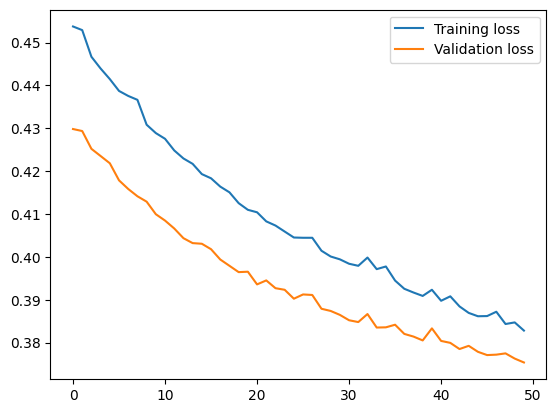
\includegraphics[width=0.55\textwidth]{yapay.png}
    \caption{5.2'deki sorunun figürü}
    \label{fig:my_pic}
\end{figure}


\subsection{(10 Puan)} \textbf{SEED=öğrenci numaranız set ettikten sonra altıncı haftada ödev olarak verdiğim gibi earlystopping'deki en iyi modeli kullanarak, Prensesi İyileştir test setinden accuracy, F1, precision ve recall değerlerini hesaplayan kodu yazın ve sonucu da aşağı yapıştırın. \%80'den fazla başarı bekliyorum test setinden. Daha düşükse başarı oranınız, nerede hata yaptığınızı bulmaya çalışın. \%90'dan fazla başarı almak mümkün (ben denedim).}

\begin{python}
train_losses = []
val_losses = []
torch.manual_seed(190401020)

for epoch in range(num_epochs):
    model.train()
    train_loss = 0.0
    for batch_idx, (data, target) in enumerate(train_loader):
        optimizer.zero_grad()
        output = model(data)
        loss = criterion(output, target.squeeze())
        loss.backward()
        optimizer.step()
        train_loss += loss.item()
    train_losses.append(train_loss/len(train_loader))

    model.eval()
    val_loss = 0.0
    correct = 0
    total = 0
    with torch.no_grad():
        for data, target in valid_loader:
            output = model(data)
            loss = criterion(output, target.squeeze())
            val_loss += loss.item()
            _, predicted = torch.max(output.data, 1)
            total += target.size(0)
            correct += (predicted == target.squeeze()).sum().item()
        val_losses.append(val_loss/len(valid_loader))
    
    accuracy = 100 * correct / total
    print('Epoch: {}, Validation Accuracy: {:.2f}%'.format(epoch+1, accuracy))
 # Check if the current accuracy is better than the best so far
    if accuracy > best_accuracy:
        best_accuracy = accuracy
        best_epoch = epoch
        torch.save(model.state_dict(), 'best_model.pt')
    # If the accuracy has not improved for the last `patience` epochs, stop training
    elif epoch - best_epoch > patience:
        print(f'Early stopping: validation accuracy has not improved for {patience} epochs.')
        break

import matplotlib.pyplot as plt

plt.plot(train_losses, label='Training loss')
plt.plot(val_losses, label='Validation loss')
plt.legend()
plt.show()

# Define the model architecture
best_model = MLP(input_size, hidden_size1, hidden_size2, output_size)
# Load the saved model
best_model.load_state_dict(torch.load("best_model.pt"))
# Set the model to evaluation mode
best_model.eval()

from sklearn.metrics import classification_report
from sklearn.metrics import accuracy_score

best_model.eval()

test_loader = DataLoader(test_dataset, batch_size=len(test_dataset), shuffle=False)
X_test, y_test = next(iter(test_loader))

with torch.no_grad():
    output = best_model(X_test)
    _, predicted = torch.max(output.data, 1)

accuracy = accuracy_score(y_test.squeeze().numpy(), predicted.numpy()) * 100
report = classification_report(y_test.squeeze().numpy(), predicted.numpy(), target_names=["Not Saved", "Saved"])

print(f"Accuracy: {accuracy:.2f}%")
print(f"Classification Report:\n{report}")
\end{python}
Epoch: 1, Validation Accuracy: 93.95\%\\
Epoch: 2, Validation Accuracy: 94.27\%\\
Epoch: 3, Validation Accuracy: 94.27\%\\
Epoch: 4, Validation Accuracy: 94.27\%\\
Epoch: 5, Validation Accuracy: 93.95\%\\
Epoch: 6, Validation Accuracy: 94.27\%\\
Epoch: 7, Validation Accuracy: 94.27\%\\
Epoch: 8, Validation Accuracy: 94.27\%\\
Early stopping: validation accuracy has not improved for 5 epochs.\\
MLP(\\
  (fc1): Linear(in_features=13, out_features=100, bias=True)\\
  (fc2): Linear(in_features=100, out_features=50, bias=True)\\
  (fc3): Linear(in_features=50, out_features=2, bias=True)\\
  (activation): ReLU()\\
)\\
Accuracy: 91.97\%\\
Classification Report:\\
   \  \    \ \  - ---  precision\ - \ recall\ - f1score  - support

   Not Saved    ----  0.91    ---  0.93 --------- 0.92 --------384\\
       Saved  --------- 0.93 -----  0.91-----------0.92---------388

    accuracy ---------------------------------- 0.92 ---------772\\
   macro avg ---------0.92-------0.92-------0.92-------772\\
weighted avg -------0.92-------0.92--------0.92-------772

\subsection{(5 Puan)} \textbf{Tüm kodların CPU'da çalışması ne kadar sürüyor hesaplayın. Sonra to device yöntemini kullanarak modeli ve verileri GPU'ya atıp kodu bir de böyle çalıştırın ve ne kadar sürdüğünü hesaplayın. Süreleri aşağıdaki tabloya koyun. GPU için Google Colab ya da Kaggle'ı kullanabilirsiniz, iki ortam da her hafta saatlerce GPU hakkı veriyor.}

\begin{table}[ht!]
    \centering
    \caption{Kodların CPU ve GPU'da çalışma süreleri}
    \begin{tabular}{c|c}
        Ortam & Süre (saniye) \\\hline
        CPU & 8.69 seconds \\
        GPU & 3.48\\
    \end{tabular}
    \label{tab:my_table}
\end{table}

\subsection{(3 Puan)} \textbf{Modelin eğitim setine overfit etmesi için elinizden geldiği kadar kodu gereken şekilde değiştirin, validasyon loss'unun açıkça yükselmeye başladığı, training ve validation loss'ları içeren figürü aşağı koyun ve overfit için yaptığınız değişiklikleri aşağı yazın. Overfit, tam bir çanak gibi olmalı ve yükselmeli. Ona göre parametrelerle oynayın.}

learning rate sayısını düşürmek ve epoch sayısını arttırmak overfit etmesine yol açıyor.

% Figür aşağı
\begin{comment}
\begin{figure}[ht!]
    \centering
    \includegraphics[width=0.75\textwidth]{mypicturehere.png}
    \caption{Buraya açıklama yazın}
    \label{fig:my_pic}
\end{figure}
\end{comment}

\subsection{(2 Puan)} \textbf{Beşinci soruya ait tüm kodların ve cevapların olduğu jupyter notebook'un Github linkini aşağıdaki url'e koyun.}

\url{https://github.com/HilalSolak/Multilayer-Perceptron_cure_the_princess/blob/main/Question5.ipynb}

\section{(Toplam 10 Puan)} \textbf{Bir önceki sorudaki Prensesi İyileştir problemindeki yapay sinir ağınıza seçtiğiniz herhangi iki farklı regülarizasyon yöntemi ekleyin ve aşağıdaki soruları cevaplayın.} 

\subsection{(2 puan)} \textbf{Kodlarda regülarizasyon eklediğiniz kısımları aşağı koyun:} 

\begin{python}
class PrincessNet(nn.Module):#Dropout yontem,
    def __init__(self):
        super(PrincessNet, self).__init__()
        self.fc1 = nn.Linear(16*16*3, 128)
        self.fc2 = nn.Linear(128, 64)
        self.fc3 = nn.Linear(64, 2)
        self.dropout = nn.Dropout(p=0.5)  #Dropout katmani

    def forward(self, x):
        x = x.view(-1, 16*16*3)
        x = nn.functional.relu(self.fc1(x))
        x = self.dropout(x)  # Dropout uygulama
        x = nn.functional.relu(self.fc2(x))
        x = self.dropout(x)  # Dropout uygulama
        x = self.fc3(x)
        return x
class PrincessNet(nn.Module):#L2 regularizasyon yontemi
    def __init__(self):
        super(PrincessNet, self).__init__()
        self.fc1 = nn.Linear(16*16*3, 128)
        self.fc2 = nn.Linear(128, 64)
        self.fc3 = nn.Linear(64, 2)

    def forward(self, x):
        x = x.view(-1, 16*16*3)
        x = nn.functional.relu(self.fc1(x))
        x = nn.functional.relu(self.fc2(x))
        x = self.fc3(x)
        return x
\end{python}

\subsection{(2 puan)} \textbf{Test setinden yeni accuracy, F1, precision ve recall değerlerini hesaplayıp aşağı koyun:}

Sonuçlar buraya.

\subsection{(5 puan)} \textbf{Regülarizasyon yöntemi seçimlerinizin sebeplerini ve sonuçlara etkisini yorumlayın:}

Seçtiğim iki regülerizasyon yöntemi olan Dropout ve L2 Regularization, aşırı öğrenmeyi engellemek için yaygın olarak kullanılan iki popüler yöntemdir.

Dropout, ağın her bir katmanında rastgele olarak belirlenen bir olasılıkla bazı nöronları geçici olarak atar ve böylece her bir eğitim örneği için farklı bir ağ elde ederiz. Bu, aşırı öğrenmeyi engellemeye yardımcı olur, çünkü nöronlar arasındaki bağlantılar rastgele kesilerek ağın daha iyi genelleştirilmesini sağlar. Bu yöntemin etkisi, eğitim verileri üzerindeki doğruluğu azaltmasına rağmen, test verileri üzerindeki performansı arttırarak daha iyi genelleştirilmiş bir model sağlayabilir.

L2 Regularization, ağdaki her bir ağırlık terimine bir ağırlık cezası ekleyerek çalışır. Bu, büyük ağırlıkların cezası daha yüksek olduğu için modelin ağırlıklarının küçük kalmasını sağlar. Bu, ağın aşırı öğrenme eğilimini azaltır ve daha iyi bir genelleştirme performansı sağlar. Aynı zamanda, ağırlık cezası parametresi olan lambda'nın doğru ayarlanması, overfitting'i önlemek için önemlidir.

Bu yöntemleri kullanarak, modelimizde aşırı öğrenmeyi önleyerek daha iyi genelleştirme performansı elde etmeyi hedefliyoruz. Bu, doğruluğu azaltabilir, ancak modelin test verileri üzerinde daha iyi performans göstermesini sağlar. Ancak, her iki yöntem de ağın daha yavaş öğrenmesine neden olabilir, bu nedenle doğru hiperparametrelerin belirlenmesi de önemlidir.

Sonuç olarak, Dropout ve L2 Regularization gibi regülerizasyon yöntemleri, aşırı öğrenme problemini çözmek için yaygın olarak kullanılan etkili yöntemlerdir. İkisi de modelin doğruluğunu azaltabilir, ancak daha iyi genelleştirilmiş bir model sağlayarak test verileri üzerinde daha iyi performans gösterirler.

\subsection{(1 puan)} \textbf{Sonucun github linkini  aşağıya koyun:}

\url{www.benimgithublinkim2.com}

\end{document}